\documentclass{standalone}
\usepackage{tikz}
\usetikzlibrary{quantikz2}
\usepackage{amsmath}

\begin{document}

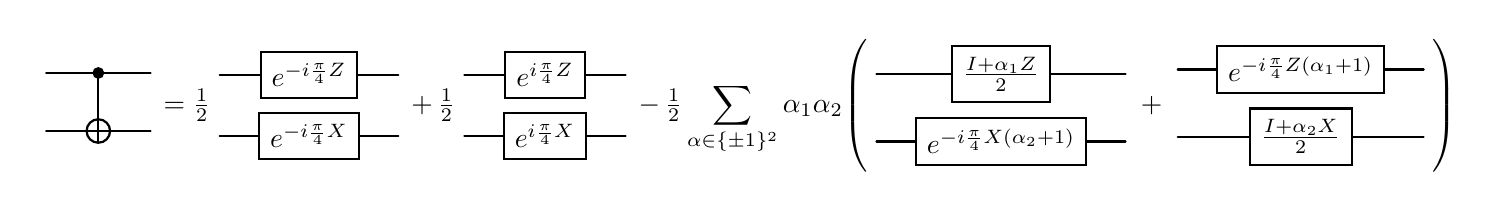
\begin{tikzpicture}[baseline=(current bounding box.center)]

% --- Left-hand side: CNOT
\node[] (lhs) {
\begin{quantikz}
&\ctrl{1} & \\
& \targ{} & 
\end{quantikz}
};

% --- First boxed circuit
\node[right=-0.2cm of lhs] (term1) {
$=\tfrac{1}{2}
\begin{quantikz}[row sep=0.2cm]
&\gate{e^{-i\frac{\pi}{4}Z} } &  \\
&\gate{e^{-i\frac{\pi}{4}X}} & 
\end{quantikz}$
};

% --- Plus second boxed circuit
\node[right=-0.2cm of term1] (term2) {
$+\, \tfrac{1}{2}
\begin{quantikz}[row sep=0.2cm]
&\gate{e^{i\frac{\pi}{4}Z}} &  \\
&\gate{e^{i\frac{\pi}{4}X}} & 
\end{quantikz}$
};

% --- Minus summation term
\node[right=-0.2cm of term2] (term3) {
$-\,\tfrac{1}{2}\displaystyle \sum_{\alpha \in \{\pm 1\}^2} \alpha_1 \alpha_2$$\left(
\begin{quantikz}[row sep=0.2cm]
&\gate{\tfrac{I+\alpha_1 Z}{2}} &  \\
&\gate{e^{-i\frac{\pi}{4}X(\alpha_2+1)} } & 
\end{quantikz}
+
\begin{quantikz}[row sep=0.2cm]
& \gate{e^{-i\frac{\pi}{4}Z(\alpha_1+1)} } &  \\
& \gate{\tfrac{I+\alpha_2 X}{2}} & 
\end{quantikz}
\right)$
};

\end{tikzpicture}

\end{document}
